\documentclass{article}\usepackage[]{graphicx}\usepackage[]{color}
%% maxwidth is the original width if it is less than linewidth
%% otherwise use linewidth (to make sure the graphics do not exceed the margin)
\makeatletter
\def\maxwidth{ %
  \ifdim\Gin@nat@width>\linewidth
    \linewidth
  \else
    \Gin@nat@width
  \fi
}
\makeatother

\definecolor{fgcolor}{rgb}{0.345, 0.345, 0.345}
\newcommand{\hlnum}[1]{\textcolor[rgb]{0.686,0.059,0.569}{#1}}%
\newcommand{\hlstr}[1]{\textcolor[rgb]{0.192,0.494,0.8}{#1}}%
\newcommand{\hlcom}[1]{\textcolor[rgb]{0.678,0.584,0.686}{\textit{#1}}}%
\newcommand{\hlopt}[1]{\textcolor[rgb]{0,0,0}{#1}}%
\newcommand{\hlstd}[1]{\textcolor[rgb]{0.345,0.345,0.345}{#1}}%
\newcommand{\hlkwa}[1]{\textcolor[rgb]{0.161,0.373,0.58}{\textbf{#1}}}%
\newcommand{\hlkwb}[1]{\textcolor[rgb]{0.69,0.353,0.396}{#1}}%
\newcommand{\hlkwc}[1]{\textcolor[rgb]{0.333,0.667,0.333}{#1}}%
\newcommand{\hlkwd}[1]{\textcolor[rgb]{0.737,0.353,0.396}{\textbf{#1}}}%

\usepackage{framed}
\makeatletter
\newenvironment{kframe}{%
 \def\at@end@of@kframe{}%
 \ifinner\ifhmode%
  \def\at@end@of@kframe{\end{minipage}}%
  \begin{minipage}{\columnwidth}%
 \fi\fi%
 \def\FrameCommand##1{\hskip\@totalleftmargin \hskip-\fboxsep
 \colorbox{shadecolor}{##1}\hskip-\fboxsep
     % There is no \\@totalrightmargin, so:
     \hskip-\linewidth \hskip-\@totalleftmargin \hskip\columnwidth}%
 \MakeFramed {\advance\hsize-\width
   \@totalleftmargin\z@ \linewidth\hsize
   \@setminipage}}%
 {\par\unskip\endMakeFramed%
 \at@end@of@kframe}
\makeatother

\definecolor{shadecolor}{rgb}{.97, .97, .97}
\definecolor{messagecolor}{rgb}{0, 0, 0}
\definecolor{warningcolor}{rgb}{1, 0, 1}
\definecolor{errorcolor}{rgb}{1, 0, 0}
\newenvironment{knitrout}{}{} % an empty environment to be redefined in TeX

\usepackage{alltt}

\title{Temperature and the Santa Ana Sucker}
\author{EA30}
\IfFileExists{upquote.sty}{\usepackage{upquote}}{}
\begin{document}


\maketitle

\newpage
\tableofcontents
\newpage

\section{Introduction}


\subsection{Problem Statement}
This report will explore whether there is a a relationship between red algae (scientific name) presence in reaches of the Santa Ana River
and the parameters of water temperature, overhead tree canopy cover, and sediment type 
 
\subsection{Background Research w/Citations} 
This project is motivated by the decline of the threatened Santa Ana sucker, a small freshwater sucker fish endemic to southern California, where it is now present in only three rivers. While there are several threats to the Santa Ana sucker, including fragmentation of its river habitats and decreasing water levels and degradation to the riparian vegetation along the river (Thomson 2010). For the Santa Ana River sucker habitat, a central threat is that the fact that the invasive Red Algae has been spreading with alacrity in areas where the fish are known to be, including the reach below the Rapid Infiltration and Extraction (RIX) Treatment plan (Los Huertos 2016).There are concerns that it may be one of the contributing factors to the suckers decline. This project will therefore focus on qualitatively identifying and analyzing the substrate on which the Algae and Red Algae found grows, because one of the aspects of the suckers habitat is the presence of coarse substrate, that is, gravel and cobble, as opposed to silt and sand (Thomson et al. 2010, 321).The sucker is adapted to feeding on the diatoms that tend to grow on the former. There is also evidence that some of the diatoms on which the sucker feeds may be able to grow on the algae (are epiphytic) (Los Huertos 2016). This may lead to the suckerbeingincontactwiththealgaewhenfeeding. Ifthesuckerisingestingthe algae, this may constitute a factor to the Suckers decline. Of course, ingesting the algae is not a necessity to the fish being negatively impacted; the algae may also disrupt the fishs well-being in unknown ways. Perhaps it actually crowds out the diatoms on which, along with algae and detritus, the sucker feeds (Thomson 2010, 322). For this reason, we will also take samples of algae found to potentially examine later for diatoms. Even if we do not detect the fish where we find algae (through collaboration with other teams who are measuring fish presence), the presence of the algae in the same area and on the same type of substrate as the fish could indicate competition for resources between the algae and the fish.


\subsection{Materials and Equipment}
Water-quality Testing instruments GPS (included in testing instruments) Foliage Testing instrument 30cm x 30cm Quadrat Water Temperature Measurer Water sediment sample bottle 10 m string/rope


\subsection{Methods}


\subsection{Site Descrition}

We evaluated 3 reaches of the Santa Ana River, with 9 observations per reach. Site A (plunge pool): 34*2’5” N, 117*21’17” W Site B (below confluence): 34*2’21” N, 117*21’20” W Site C (above confluence): 34*2’29” N, 117*21’15” W. Each observation contains the following variables: algae percent cover, canopy cover, water temperature, bed composition. near Colton, California (Figure \ref{SAR_Image}). 

\begin{figure}
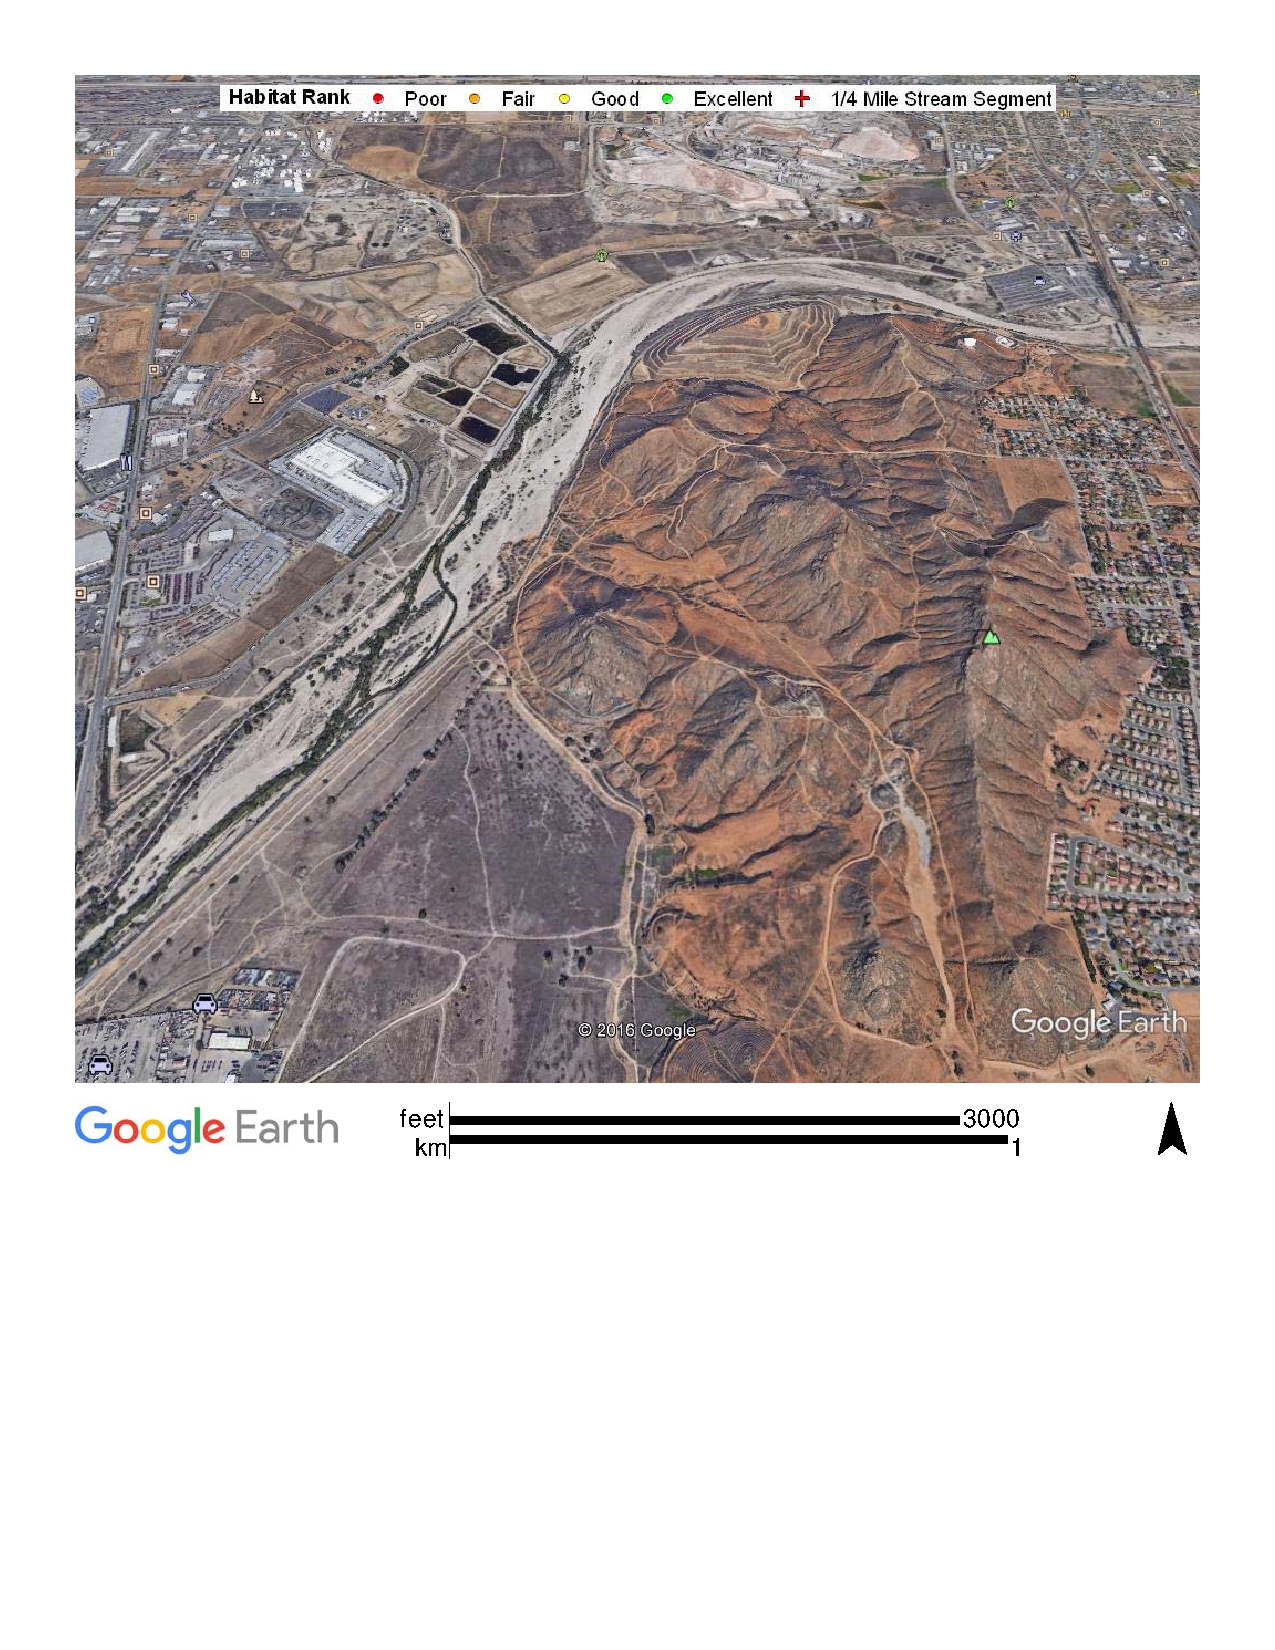
\includegraphics[width=1.00\textwidth]{Figures/SantaAna_SatelliteImage}
\caption{Google Earth --THIS IS HOW YOU DO A CAPTION IN CASE WE NEED IT}
\label{SAR_Image}
\end{figure}

\subsection{Field Methods}
Site selection: 3 measurements 1-10m apart for 4 different reaches. Use random number generator to select distance. 12 measurements total. Reach 1 = original site visited already. Must select Reaches 2 3 in between. Reach 4 = fish-rich pool half hour downstream 30 minutes to walk down to reach D where we will start, then proceed back upstream. ATEACHSITE(25minuteseach): Algae: usequadrat30cmx30cm. Take three measurements on right bank, middle, left bank. For each measurement, estimate Pebble count. (What was the pebble structure and was the algae on the pebbles) Pebble size: qualitatively note grain size of streambed: cobbles, pebbles, coarse sand, fine sand, or silt. Canopy cover: directly above each alage measurement, use canopy cover instrument to determine canopy cover. Temperature: 3 measurements per site, left middle and right. Time of each measurement Notekeeper who records as team members call out measurements TOTAL TIME NEEDED: 2 hours 40 mins
\subsection{Laboratory Methods}

\subsection{Statistical Methods}
After conducting our fieldwork, we will enter our data in rstudio. We will produce linear regressions of temperature vs algae abundance. We will producelinear regressions of canopy cover vs algae abundance. We will produce linear regressions of canopy cover vs temperature. We will create ANOVA or t-tests of bed composition vs. algae abundance. We will then analyze our data and write a project report 4-5 pages long with pictures and figures. We should hopefully be able to draw conclusions about canopy cover, temperature, and stream bed compositions effect on algae abundance. In qualitative terms, we will synthesize our results with the fish videography team and state whether our observed relationship between stream conditions and algae abundance matches the frequency of their fish observations.

\section{Results}

The temperature data suggests... (Figure \ref{Temp}).

\begin{figure}
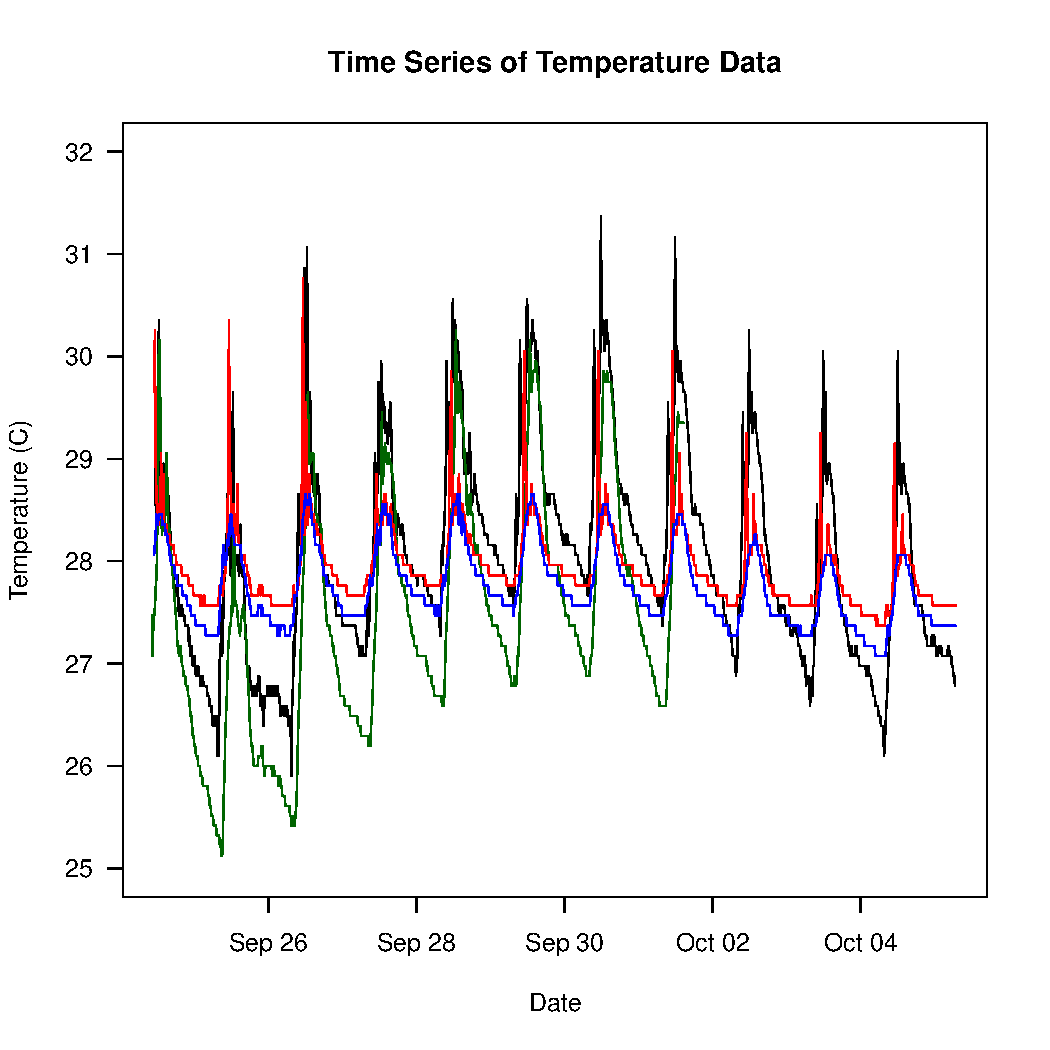
\includegraphics{Figures/Temp}
\caption{Temperature time...}
\label{Temp}
\end{figure}

\section{Discussion}


\section{Conclusion and Recommendations}


\end{document}
